\documentclass[a4paper,12pt]{article}

\usepackage{amsmath,amssymb,multicol,tikz,enumitem}
\usepackage[margin=2cm]{geometry}
%\usetikzlibrary{calc}
\usepackage{amsmath}
\usepackage{amsthm}
\usepackage{thmtools}
\usepackage{hyperref}
\usepackage{enumerate}
\usepackage{xcolor}

\pagestyle{empty}

\newcommand\Q{\mathbf{Q}}
\newcommand\R{\mathbf{R}}
\newcommand\Z{\mathbf{Z}}

\newcommand\answer[1]{}
\newcommand\ans[1]{}
%\newcommand\answer[1]{\\[5pt]{\color{blue}{#1}}\hfill{\color{blue}}\\[-5pt]} 
%\newcommand\ans[1]{{\color{blue}{#1}}}

\usepackage{array}
\newcolumntype{P}[1]{>{\centering\arraybackslash}p{#1}}

\newcommand\indd{${}$\hspace{20pt}}

\declaretheoremstyle[headfont=\normalfont\bfseries,notefont=\mdseries\bfseries,bodyfont = \normalfont,headpunct={:}]{normalhead}
\declaretheorem[name={Uzdevums}, style=normalhead,numberwithin=section]{problem}

\setcounter{section}{01}

\setlength\parindent{0pt}

\renewcommand{\figurename}{Attēls}

\begin{document}

\begin{center}
\parbox{3.5cm}{\flushleft\bf Dalāmība, Pirmskaitļi, LKD un MKD} \hfill {\bf\LARGE Sacensības \#2021.01} \hfill \parbox{3.5cm}{\flushright\bf 2021-02-18} \\[2pt]
{\rm\footnotesize Par šo LU NMS atbalstīto pasākumu\\ atbild {\tt kalvis.apsitis@gmail.com}.}
\end{center}

%\hrule\vspace{2pt}\hrule
\hrule

%\vspace{10pt}
%{\bf Iesniegšanas termiņš:} 2021.g.\ 20.februāris\\
%{\bf Kam iesūtīt:} {\tt kalvis.apsitis}, domēns {\tt gmail.com}

%{\large\bf Eratostēna režģis.} 

\vspace{10pt}
\begin{figure}[!htb]
\center{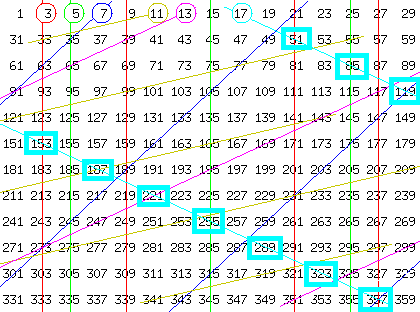
\includegraphics[width=3in]{online-competition-2021-02-18/eratosthenes-with-17.png}}
\caption{\label{fig:eratosthenes-with-17} Eratostēna režģis nepāru skaitļiem.}
\end{figure}

\vspace{10pt}
\begin{problem}
Eratostēnam patīk veidot režģus šādi: Visus nepāra skaitļus viņš izkārto 
rindās pa $15$; tad velk taisnes, uz kurām atrodas saliktie skaitļi, 
kas dalās ar $3$, $5$, $7$, utt. Attēlā ar taisnstūrīšiem apvilkti visi 
nepāru saliktie skaitļi, kas dalās ar $17$ 
(tie ir $51$,$85$,$119$,$153$,$187$, $\ldots$).
Pieņemsim, ka pēdējais skaitlis Eratostēna režģī ir $8999$
(attēlā redzama tikai režģa augšdaļa).

{\bf Jautājums:} Cik daudzi ar taisnstūrīti apvilkti skaitļi 
atradīsies tajā Eratostēna režģa kolonnā, 
kurā to ir vismazāk? Ierakstiet atbildē naturālu skaitli.
(Par kolonnu saucam vertikāli, kur skaitļi rakstīti 
viens zem otra. Piemēram $1,31,\ldots$ vai $3,33,\ldots$.)
\answer{

{\bf Atbilde:} $\mathtt{17}$\\
{\bf ``Vienmērības'' Lemma:} Nepāra skaitļi, 
kuri dalās ar $17$ (ir apvilkti ar taisnstūrīti) visas vertikāles aizpilda 
``vienmērīgi'': Tas nozīmē to, ka jebkura vertikāle saņem otro taisnstūrīti 
tikai pēc tam, kad {\bf visas} vertikāles jau saņēmušas pirmo taisnstūrīti; 
jebkura vertikāle saņem trešo taisnstūrīti tikai pēc tam, kad visas jau saņēmušas otro utt. 
(Attēlā~\ref{fig:eratosthenes-with-17} nākamie ar taisnstūri apvilktie skaitļi 
nonāks 1.,3.,5.,7. kolonnā, kuras šobrīd ir tukšas, utt.)

Pierādījums seko no tā, ka aritmētiskajā progresijā 
\begin{equation}
\label{eq1:progression}
a_n = 51+34(n-1)
\end{equation}
(nepāra skaitļi, kas dalās ar $17$)
jāpieskaita tieši $15$ diferences $d=34$, lai atgrieztos tajā pašā kolonnā
(pirms tam ``izstaigājot'' visas citas kolonnas, jo arī tajās aritmētiskā progresija 
nonāk ne biežāk kā reizi $15$ soļos). Mūsu gadījumā 
\[ a_1 = 51 \equiv a_{16} = 561 \pmod{15}. \]
Šāds ``vienmērīgums'' seko no tā, ka $\text{LKD}(34,15)=1$. 
Tie skaitļi, kuri dalās ar $3$ un ar $5$ (kam ir kopīgi dalītāji ar $15$), nav 
izvietoti kolonnās vienmērīgi (sk. vertikālās sarkanās un zaļās taisnes zīmējumā). $\blacksquare$


{\bf Intuīcija:} 
Katra tabulas rinda attēlo nepāra skaitļus no $[1;30]$; $[31;60]$ utt. 
Pavisam tabulā ir $9000/30 =  300$ šādu rindu; pa $15$ nepāra skaitļiem katrā. 
Katrs septiņpadsmitais no tiem ir ar taisnstūrīti. ``Vienmērības'' īpašības 
dēļ daļā no kolonnām būs $\lfloor 300/17 \rfloor = \lfloor 17.64706 \rfloor = 17$ 
taisnstūrīši (ar $\lfloor x \rfloor$ apzīmēta apakšējā veselā daļa). Citās kolonnās būs $17+1=18$ taisnstūrīši. 

{\bf Formāls atbildes pamatojums:} 
Pirmais nepāru saliktais skaitlis, kas dalās ar $17$ ir aritmētiskās progresijas (\ref{eq1:progression}) loceklis
$a_1 = 51$  (pats $17$ ir pirmskaitlis, 
tam nav sava taisnstūrīša); pēdējais ir $a_{264} = 8993$, jo $8993 = 17\cdot \lfloor 9000/17 \rfloor$
ir lielākais skaitlis no $[1;9000]$, kas dalās ar $17$

``Vienmērības lemmas'' dēļ visi 264 aritmētiskās progresijas locekļi sadalās pa $15$ kolonnām vienmērīgi 
(taisnstūrīšu skaits dažādās kolonnās nevar atšķirties vairāk kā par $1$). Skaitli $264$ tikai vienā veidā
var izteikt kā $15$ skaitļu summu, ievērojot šo nosacījumu:
\[ 264 = \underbrace{18+18+18+18+18+18+18+18+18}_{9\ \text{saskaitāmie}} + \underbrace{17+17+17+17+17+17}_{6\ \text{saskaitāmie}}. \]
Tādēļ tajās sešās kolonnās, kur taisnstūrīšu ir mazāk kā citās, to būs $17$ (bet pārējās deviņās kolonnās būs pa $18$). 
}
\end{problem}





\vspace{20pt}
\begin{problem}
Tabulā attēloti veselie skaitļi $[5041;5160]$. 
Pirmajā solī izsvītro visus pāra skaitļus; otrajā solī \textendash{} visus skaitļus, 
kuri dalās ar $3$; trešajā solī \textendash{} visus skaitļus, kuri dalās ar $5$. 
Cik skaitļi palika neizsvītroti pēc šiem trim soļiem (citiem vārdiem, 
cik daudzi $x \in [5041;5160]$ nedalās ne ar vienu no skaitļiem $2$, $3$ vai $5$.

{\bf Jautājums:} Ierakstīt atbildē neizsvītroto skaitļu skaitu.
\answer{

{\bf Atbilde:} $\mathtt{32}$\\
Skaitļu intervāla garums ir $120$; no tā izsvītro visus tos skaitļus, kuriem ir 
kopīgi dalītāji ar $120$. Izsvītroto skaitļu daudzums nemainīsies, ja 
no katra intervāla skaitļa atņems nobīdi $5040$.

{\bf Apgalvojums.} Katram naturālam $x$, skaitlis $x + 5040$ dalās ar $2$
(attiecīgi ar $3$, vai ar $5$) tad un tikai tad, ja pats $x$ dalās ar $2$
(attiecīgi ar $3$, vai ar $5$). 

Apgalvojumu var pamatot ar to, ka pati nobīde $5040$ dalās ar $2 \cdot 3 \cdot 5 = 30$. 
Tāpēc neizsvītroto skaitļu būs pavisam 
\[ \varphi(120) = 120 \cdot \left( 1 - \frac{1}{2} \right) \cdot\left( 1 - \frac{1}{3}  \right) \cdot\left( 1 - \frac{1}{5}  \right) 
= 120 \cdot \frac{1}{2} \cdot \frac{2}{3} \cdot \frac{4}{5} = 32. \]
(Sākumā ir $120$ skaitļi, vispirms izsvītro katru otro (paliek puse), 
tad katru trešo (paliek divas trešdaļas no vēl neizsvītrotajiem) un visbeidzot katru piekto (paliek četras piektdaļas). 

}
\end{problem}


\vspace{20pt}
\begin{problem}
Sienāzis sākumā atrodas punktā ar koordinātēm $(0;0)$. 
Vienā gājienā tas var pārvietoties no punkta $(x;y)$ uz kādu no četriem 
punktiem $(x - 35; y - 12)$, $(x + 35; y + 12)$, $(x-12; y+35)$ vai 
$(x+12; y-35)$. 
Pēc kāda laika sienāzis nonāk punktā $(1;y)$. Atrast mazāko pozitīvo $y$, kam tas ir iespējams.

{\bf Jautājums:} Ierakstīt atbildē naturālu skaitli: mazāko $y$ ar minēto īpašību. 
\answer{

{\bf Atbilde:} $\mathtt{1252}$\\
Tā kā $\text{LKD}(35,12)=1$, tad izpildās Bezū identitāte: Eksistē veseli skaitļi $x,y$, kam
\[ 35x + 12y = 1.\;\;\text{Piemēram, $x=-1$, $y=3$.} \]
Ja sienāzis vienreiz izmantos gājienu $(x;y) \Rightarrow (x - 35; y-12)$, bet pēc tam trīsreiz gājienu 
$(x;y) \Rightarrow (x+12; y-35)$, tad pārvietošanās izskatās šādi:
\[ (0;0) \;\Rightarrow\; (-35;-12) \;\Rightarrow\; (-23;-47) \;\Rightarrow\; (-11;-82) \;\Rightarrow\; (1;-117). \]
Šādi var panākt, lai jaunā $x$ koordināte būtu $0 - 35 + 3 \cdot 12 = 1$. Diemžēl, $y$ koordināte nav pozitīva.

Lai sienāzis iegūtu pozitīvu $y$ koordināti, tas var no $(0;0)$ pārvietoties $11$ soļus pa lēcienu $(x + 35; y + 12)$, 
bet pēc tam $32$ reizes pa lēcienu $(-12; +35)$:
\[ (0;0) \;\Rightarrow\; 11 \cdot (35;12) + 32 \cdot (-12; +35) = 
(11 \cdot 35 + 32\cdot(-12); 11\cdot{}12 + 32\cdot{}35 = (1;1252). \]

Sienāzis nevar izmantot lēcienu $(x + 35; y + 12)$ mazāk kā $11$ reizes, jo
pie $k=1,\ldots,10$, skaitlim $35k$ nebūs atlikums $1$, dalot ar $12$. 
Lai atrastu visus atrisinājumus vienādojumam $35x-12y=1$, var izmantot 
Eiklīda algoritmu (meklēt LKD skaitļiem $35$ un $12$, lai atrastu 
veidus, kā izteikt $LKD(35,12)=1$). Var arī izmantot WolframAlpha 
\cite{WolframAlpha} vienādojumu risinātāju; tur ir redzami arī atrisinājumi 
veselos skaitļos:

\vspace{20pt}
\begin{figure}[!htb]
\center{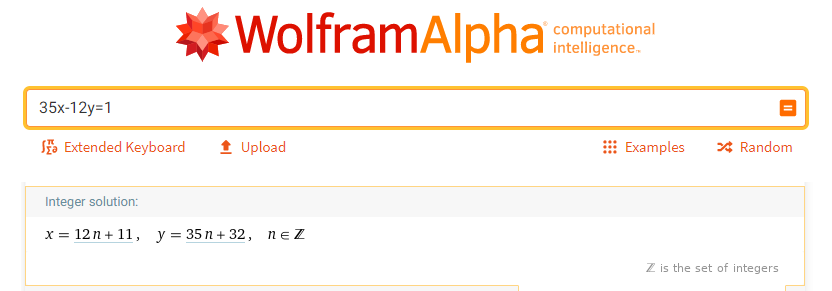
\includegraphics[width=5in]{online-competition-2021-02-18/wolfram-alpha.png}}
\caption{\label{fig:wolfram-alpha} WolframAlpha atrisinājums vienādojumam.}
\end{figure}
}
\end{problem}



%(12, 35, 37)
% 11*12 + 32*35 = 
%> (1 + 2 + 4 + 8)*(1 + 3 + 9)*(1 + 5)
%[1] 1170
%> (1 + 2 + 4 + 8)*(1 + 3)*(1 + 5 + 25)
%[1] 1860
%> 1170 + 1860 - 360
%[1] 2670




\vspace{20pt}
\begin{problem}
%%            35   36       20  21       2k=20  7m 2k+2
%%  14 ...    7    2        2   7        2      7  2
%%  15 ...    5    3        5   3        5      3  1
Atrast mazāko $x$ vērtību, kurai 
visi skaitļi $\text{LKD}(14,x)$, $\text{LKD}(14,x+1)$, $\text{LKD}(15,x)$ un $\text{LKD}(15,x+1)$ ir lielāki par $1$. 

{\bf Jautājums:} Ierakstīt naturālu skaitli $x$ ar šo īpašību.
\answer{

{\bf Atbilde.} $\mathtt{20}$\\
Lai minētās LKD vērtības nebūtu $1$, abi skaitļi $14$ un $15$ nevar būt savstarpēji pirmskaitļi ne ar $x$, ne ar $x+1$
(tas viss neraugoties uz to, ka paši $14$ un $15$ ir savstarpēji pirmskaitļi; arī $x$ un $x+1$ tādi ir). 

Tā kā $14 = 2 \cdot 7$ un $15 = 3 \cdot 5$, tad $x$ un $x+1$ (pa abiem kopā) satur šos pašus četrus pirmreizinātājus, 
tikai citādi sakombinētus.

{\bf 1.gadījums.} $x$ dalās ar $2 \cdot 5$ un $x+1$ dalās ar $3 \cdot 7$ (maxākais atrisinājums $x = 20$, $x+1 = 21$.\\
{\bf 2.gadījums.} $x$ dalās ar $3 \cdot 7$ un $x+1$ dalās ar $2 \cdot 5$ (mazākais atrisinājums $x = 189$, $x+1 = 190$.\\
{\bf 3.gadījums.} $x$ dalās ar $5 \cdot 7$ un $x+1$ dalās ar $2 \cdot 3$ (maxākais atrisinājums $x = 35$, $x+1 = 36$.\\
{\bf 4.gadījums.} $x$ dalās ar $2 \cdot 3$ un $x+1$ dalās ar $5 \cdot 7$ (mazākais atrisinājums $x = 174$, $x+1 = 175$.

No visiem minētajiem gadījumiem vismazākais ir $x = 20$, kas arī ir mūsu atbilde.
}
\end{problem}
% x = 20
% 4028



\vspace{20pt}
\begin{problem}
Aprēķināt summu $\text{LKD}(10!,1) + \text{LKD}(10!,2) + \text{LKD}(10!,3) + \ldots + \text{LKD}(10!,100)$, 
kur saskaita lielākos kopīgos dalītājus skaitlim $10!$ (desmit faktoriāls) ar pirmajiem $100$ naturālajiem skaitļiem. 
\answer{

{\bf Atbilde:} $\mathtt{1846}$\\
Daudziem $n \in [1;100]$ ir spēkā $\text{LKD}(10!,n) = n$, jo $10!$ dalās ar $n$. 
Tāpēc ``pirmo tuvinājumu'' iegūstam, summējot skaitļus no $1$ līdz $100$, iegūstot 
\begin{equation}
\label{eq:sum-to-100}
1 + 2 + 3 + \ldots + 99+ 100 = \frac{100 \cdot 101}{2} = 5050.
\end{equation}
%Tomēr visiem pirmskaitļiem $p>10$ izpildīsies $\text{LKD}(10!,p) = 1$ un 
%arī $\text{LKD}(10!,p \cdot k) = k$ (katram $k < 10$). 
%Teiksim, skaitlim $11 \cdot 9$, LKD būs $9$ (mazāk par pašu 99).

Aplūkojam skaitļus $n = 11k$ ($n=11,22,33,\ldots,99$). Piemēram, $\text{LKD}(10!,99)=9$ (jo $10!$ nedalās ar $11$), 
bet izteiksmē (\ref{eq:sum-to-100}) jau esam pieskaitījuši nevis $9$, bet $99$. 
Tāpēc summai $5050$ jāpieskaita negatīva ``korekcija'': $(9 - 99)$. Sagrupējam visas korekcijas 
skaitļiem ($n=11,22,33,\ldots,99$):\\
\mbox{}\hspace{1cm} $(1 - 11) + (2-22) + \ldots + (9 - 99) =$\\
\mbox{}\hspace{1cm} $= (1 + 2 + \ldots + 9) - (11 + 22 + \ldots + 99) = 45 - 45 \cdot 11 = 45 \cdot (-10).$

Līdzīgi darām arī tiem, kas dalās ar $13$ (t.i. $n=13,26,\ldots,91$); arī skaitļiem, kas dalās ar $p = 17,19,23,29,31$. 
Izrakstām visas korekcijas.

{\small
\[ \begin{array}{ll}
\text{Ja $p = 13$, tad}\ & (1 + 2 + \ldots + 7) - (13 + 26 + \ldots + 91) = 28 - 28 \cdot 13 = 28 \cdot (-12) \\
\text{Ja $p = 17$, tad}\ & (1 + 2 + 3+ 4 + 5) - (1 + 2 + 3+ 4 + 5) \cdot 17 = 15 - 15 \cdot 17 = 15 \cdot (-16) \\
\text{Ja $p = 19$, tad}\ & (1 + 2 + 3 + 4 + 5) - (1 + 2 + 3+ 4 + 5) \cdot 19 = 15 - 15 \cdot 19 = 15 \cdot (-18) \\
\text{Ja $p = 23$, tad}\ & (1 + 2 + 3 + 4) - (1 + 2 + 3+ 4) \cdot 23 = 10 - 10 \cdot 23 = 10 \cdot (-22) \\
\text{Ja $p = 29$, tad}\ & (1 + 2 + 3) - (1 + 2 + 3) \cdot 29 = 6 - 6 \cdot 29 = 6 \cdot (-28) \\
\text{Ja $p = 31$, tad}\ & (1 + 2 + 3) - (1 + 2 + 3) \cdot 31 = 6 - 6 \cdot 31 = 6 \cdot (-30) \\
\end{array}
\]
}

Ja $p=37, 41, 43, 47$, tad katram no tiem jāpieskaita $(1+2)$, bet jāatņem $(1+2)\cdot p$. Iegūstam
\[ (1 + 2) \cdot 4 - (1 + 2) \cdot (37 + 41 + 43 + 47) = -492 \]
Visbeidzot, ja $p = 53,59,61,67,71,73,79,83,89,97$, tad LKD summas korekcija ir 
\[ 1 \cdot 10 - (53 + 59 + 61 + 67 + 71 + 73 + 79 + 83 + 89 + 97) = -722. \]

Pieskaitām šīs izmaiņas:\\
{\small
$5050 + 45 \cdot (-10) + 28 \cdot (-12) + 15 \cdot (-16) + 15 \cdot (-18) + 10 \cdot (-22) + 6 \cdot (-28) + 6 \cdot (-30) - 492 - 722 = 1972.$
}

Ja $n=49$ vai $n=98$, tad $\text{LKD}(10!,49) = 7$ un $\text{LKD}(10!,98) = 14$; tātad pieskaitām vēl divas negatīvas korekcijas: 
$1972 + (7-49) + (14 - 98) = 1846$.

Neviens skaitlis no $[1;100]$ nevar dalīties ar vairākiem pirmskaitļiem (vai arī $49,98$), 
tāpēc skaitļu atkārtošanās šajās korekcijās nav iespējama.
}
\end{problem}
% 5050 - 11 - 13 - 17 - 19 - 23 - 29 - 31 - 37 - 41 - 43 -   47 - 53 - 59 - 61 - 67 - 71 - 73 - 79 - 83 - 89 - 97 + 21
%


\vspace{10pt}
\begin{problem}
Anna saliek $600$ akmentiņus $m$ kastītēs tā, ka ikvienā kastītē ir vienāds skaits dārgakmeņu. 
Kastīšu ir vairāk nekā viena un katrā kastītē ir vairāk nekā viens akmentiņš. 
Cik dažādām $m$ vērtībām to var izdarīt?
\answer{

{\bf Atbilde:} $\mathtt{22}$\\
Skaitļa $600$ sadalījums pirmreizinātājos ir $600 = 2^3 \cdot 3^1 \cdot 5^2$.
(Citiem vārdiem, $600  = p_1^{a_1} \cdot p_2^{a_2} \cdot p_3^{a_3}$, kur $p_1 = 2$, $p_2 = 3$, $p_3 = 5$, bet 
$a_1 = 3$, $a_2 = 1$, $a_3 = 2$.)

Tādēļ pozitīvo dalītāju skaits skaitlim $600$ ir (izmantojam formulu no \cite{Raji2020}):
\[ \sigma_0(600) = \sum\limits_{d \mid 600} 1 = \prod\limits_{i=1}^{3} (a_i+1) = (3 + 1)(1+1)(2+1) = 4 \cdot 2 \cdot 3 = 24. \]
Neder tie gadījumi, kad kastīšu skaits $m=1$ vai $m=600$. Atliek $24 - 2 = 22$ iespējas skaitļa $m$ vērtībai.


}
\end{problem}

\vspace{20pt}
\begin{problem}
Atrast visu to skaitļu $d$ summu, kuriem $d \mid 360$ un $d \mid 600$
(t.i.\ $d$ ir skaitļa $360$ {\bf un} skaitļa $600$ dalītājs).
\answer{
% (1 + 2 + 4 + 8)*(1 + 3)*(1 + 5)

{\bf Atbilde:} $\mathtt{360}$\\
Skaitļi $d$ ir precīzi tie, kuri ir skaitļa $\text{LKD}(360,600) = 120$
dalītāji. 
Sadalām pirmreizinātājos: $120  = p_1^{a_1} \cdot p_2^{a_2} \cdot p_3^{a_3} = 2^3 \cdot 3^1 \cdot 5^1$. 

Skaitļa $120$ dalītāju summa ir (izmantojam formulu no \cite{Raji2020B}):
\[ \sigma_1(120) = \sum\limits_{d \mid 120} d =  \prod\limits_{i=1}^{3} (p_i^{a_i}+ p_i^{a_i-1} + \ldots + p_i +1) = (1 + 2 + 4 + 8)\cdot{}(1 + 3)\cdot{}(1 + 5) = 360. \]
}
\end{problem}
\vspace{20pt}
\begin{problem}
Atrast visu to skaitļu $d$ summu, kuriem $d \mid 360$ vai $d \mid 600$
(t.i.\ $d$ ir skaitļa $360$ {\bf vai} skaitļa $600$ dalītājs).
\answer{

% (1 + 2 + 4 + 8)*(1 + 3 + 9)*(1 + 5)

{\bf Atbilde:} $\mathtt{2670}$\\
Dalām pirmreizinātājos: 
\[ \left\{ \begin{array}{l}
120 = 2^3 \cdot 3^1 \cdot 5^1,\\
360 = 2^3 \cdot 3^2 \cdot 5^1,\\
600 = 2^3 \cdot 3^1 \cdot 5^2.\\
\end{array} \right. \]
Izmantojot formulu no \cite{Raji2020B}, iegūstam
\[ \left\{ \begin{array}{l}
\sigma_1(120) = (1 + 2 + 4 + 8)\cdot{}(1 + 3)\cdot{}(1 + 5) = 360,\\
\sigma_1(360) = (1 + 2 + 4 + 8)\cdot{}(1 + 3 + 9)\cdot{}(1 + 5) = 1170,\\
\sigma_1(600) = (1 + 2 + 4 + 8)\cdot{}(1 + 3)\cdot{}(1 + 5 + 25) = 1860.\\
\end{array} \right. \]
Lai atrastu tos skaitļus, kuri dalās ar $360$ vai $600$, varam saskaitīt $1170+1860$, bet 
tie $d$, kuri ir abu šo skaitļu dalītāji (tātad arī skaitļa $120 = \text{LKD}(360,600)$ dalītāji), 
ir ieskaitīti divas reizes. Tāpēc no šīs summas jāatņem $360$: 
\[ 1170 + 1860 - 360 = 2670. \]
}
\end{problem}

\vspace{20pt}
\begin{problem}
Ar faktoriāla palīdzību var konstruēt cik patīk garus intervālus, kuros nav neviena pirmskaitļa.
Piemēram, ir zināms, ka intervālā $[14!+2,\ldots,14!+14]$ ir $13$ pēc kārtas sekojoši salikti skaitļi.
Atrast līdzīgu intervālu $[x,x+12] \subseteq [100;200]$, kurā arī ir $13$ skaitļi, no kuriem neviens nav pirmskaitlis.

{\bf Jautājums:} Ierakstīt skaitli $x$, kur $x$ ir pirmais saliktais skaitlis trīspadsmit saliktu skaitļu virknē.
\answer{

{\bf Atbilde:} $\mathtt{114}$\\
Ar tiešām pārbaudēm varam pārliecināties, ka visi trīspadsmit skaitļi intervālā $[114;126]$ ir salikti.

{\em Piezīme.} Atstarpes starp pirmskaitļiem minētas šajā tabulā: \cite{UTMprimeGaps}.
}
\end{problem}
%https://primes.utm.edu/notes/GapsTable.html




%\vspace{20pt}
%\begin{problem}
%Atrast tādu mazāko $y$, kur dotajam $x=\ldots$ būs spēkā vienādība $LKD(y,x)\cdot LKD(y,x+1)\cdot  LKD(y,x+2) \cdot  LKD(y,x+3) = y^2$. 
%\end{problem}


\vspace{20pt}
\begin{figure}[!htb]
\center{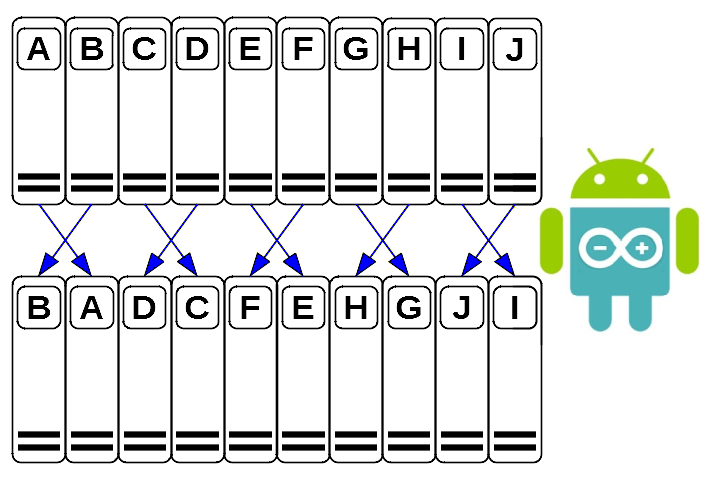
\includegraphics[width=2.6in]{online-competition-2021-02-18/robot-and-books.png}}
\caption{\label{fig:robot-and-books} Sējumu pārkārtošana.}
\end{figure}

\vspace{10pt}
\begin{problem}
Karantīnas dēļ bibliotēkā drīkst uz\-tu\-rē\-ties vienīgi robots.
Plauktā ir $10$ enciklopēdijas sējumi, kas apzīmēti ar burtiem $A,\ldots,J$,
pašā sākumā tie sakārtoti pēc alfabēta.
Reizi stundā robots sējumus pārkārto:
sējumu, kurš atradās pirmajā vietā, noliek
vie\-tā $n_1$, $\ldots$, sējumu, kurš atradās desmitajā vietā, noliek vietā
$n_{10}$. ($n_1,\allowbreak\ldots,\allowbreak{}n_{10}$ ir dažādi
naturāli skaitļi no $1$ līdz $10$ \textendash{} tie robota dzīves laikā paliek nemainīgi.)

Pēc tieši $T$ šādām pārkārtošanām sējumi atkal sakārtojas sākotnējā al\-fa\-bē\-tis\-kajā 
secībā. Atrast lielāko perioda $T$ vērtību. Piemēram attēlā 
redzamajam robotam, kurš vienkārši blakusesošos sējumus apmaina vietām, $T=2$. 

{\bf Jautājums:} Ierakstīt naturālu skaitli: lielāko iespējamo perioda vērtību.
\answer{

{\bf Atbilde:} $\mathtt{30}$ (\textcolor{orange}{1 punkts}).\\
{\bf Daļējās atbildes.} Var dabūt arī periodus $\mathtt{12}$, $\mathtt{15}$ vai $\mathtt{21}$ (\textcolor{orange}{0.5 punkts}).\\
Grāmatu pārkārtošanu atbilstoši vienam un tam pašam musturam, kurā norādīts,
uz kuru vietu pārceļ katru no grāmatām, sauc par saraksta {\em permutāciju}.
Desmit grāmatām ie\-spē\-ja\-mas pavisam $10! = 3628800$ (tik veidos
var ieprogrammēt grāmatu jaukšanas robotu).

Permutācijām var veidot {\em kompozīcijas}, tās pie\-lie\-to\-jot vienu pēc otras
(vispirms pārkārto pēc viena mustura, tad pēc otra).
Starp visām permutācijām īpaša loma ir {\em vienības permutācijai}, kura atstāj
visas grāmatas uz vietas. Mūs interesē, cik reizes permutācija ``jāreizina'' pati ar sevi, lai 
iegūtu vienības permutāciju (to sauksim par {\em permutācijas kārtu} jeb {\em order of a permutation}).

{\bf Definīcija} Katrai permutācijai par {\em ciklu} sau\-cam tādu grāmatu virkni
ar numuriem\\ $a_1,\ldots,a_n$, kas šajā permutācijā mainās ``pa apli'':
$a_1$ nonāk vietā $a_2$, $a_2$ nonāk $a_3$,
utt. Visbeidzot $a_n$ nonāk $a_1$.
Ja grāmata paliek uz vietas, to raksta kā ciklu garumā $1$.

{\bf Apgalvojums.} Ikviena permutācija izsakāma kā viena vai vairāku ciklu kompozīcija, 
kur cikliem nav kopīgu elementu.\\
{\bf Piemērs.} Aplūkosim šādu ``nejaušu'' permutāciju:\\
\begin{tabular}{|l|c|c|c|c|c|c|c|c|c|c|} \hline
No kurienes & 1 & 2 & 3 & 4 & 5 & 6 & 7 & 8 & 9 & 10 \\ \hline
Uz kurieni & 10 & 1 & 5 & 7 & 6 & 8 & 9 & 3 & 4 & 2 \\ \hline
\end{tabular}\\
Grāmata no vietas \#1 vispirms ceļo uz vietu \#10, tad uz vietu \#2, visbeidzot atpakaļ uz \#1. 
Tāpēc $(1,10,2)$ ir viens cikls. Pavisam tur ir šādi cikli: 
\[ (1,10,2),\;\;(3,5,6,8),\;\;(4,7,9). \]
Šajā piemērā pēc $T=3 \cdot 4 = 12$ soļiem
visas grāmatas būs izgājušas veselu skaitu ciklu un atgriezušās sākotnējās pozīcijās.

Lai izveidotu permutāciju ar iespējami lielu kārtu, apvienosim vienā kompozīcijā vairākus
ciklus, kuru garumi ir savstarpēji pirmskaitļi (tad elementa kārta būs visu šo ciklu garumu
reizinājums). Piemēram, ja permutācijā pie\-cas grāmatas veido vienu ciklu, trīs citas grāmatas
otru ciklu, visbeidzot atlikušās divas vēl vienu ciklu, tad
šāda elementa kārta būs $5 \cdot 3 \cdot 2 = 30$.

Varam, piemēram, ``pa apli'' mainīt grāmatas šādos ciklos: 
$(A,\allowbreak{}B,\allowbreak{}C,\allowbreak{}D,\allowbreak{}E)$, $(F,\allowbreak{}G,\allowbreak{}H)$ un arī $(I,\allowbreak{}J)$.
Pārrakstot šo par robota programmu:

\vspace{4pt}
\begin{tabular}{|l|c|c|c|c|c||c|c|c||c|c|} \hline
No kurienes & 1 & 2 & 3 & 4 & 5 & 6 & 7 & 8 & 9 & 10 \\ \hline
Uz kurieni & 2 & 3 & 4 & 5 & 1 & 7 & 8 & 6 & 10 & 9 \\ \hline
\end{tabular}

{\em Piezīme 1.} Šī ir parodija par {\em University of Albany} pasniedzēja
Antun Milas analizētu kontroldarbu \cite{Milas2015}.

{\em Piezīme 2.} Mazā Fermā teorēma arī nosaka kārtas noteikta veida permutācijām (reizināšanai ar $a$ pēc 
$\pmod{p}$). Piemēram, pirmskaitlim $p=11$, reizināšanu ar skaitli $3$ attēlo sekojoša permutācija:\\
\begin{tabular}{|l|c|c|c|c|c|c|c|c|c|c|} \hline
No kurienes & 1 & 2 & 3 & 4 & 5 & 6 & 7 & 8 & 9 & 10 \\ \hline
Uz kurieni & 3 & 6 & 9 & 1 & 4 & 7 & 10 & 2 & 5 & 8 \\ \hline
\end{tabular}\\
Uzrakstīta ar cikliem, tā izskatās šādi: 
\[ (1,3,9,5,4),\;\;(2,6,7,10,8). \] 
Mazā Fermā teorēma apsola, ka šādām īpašām permutācijām kārta vienmēr ir $p-1 = 10$ 
vai arī tā dala skaitli $p-1$. Piemēram, skaitļa $3$ multiplikatīvā kārta $\pmod{11}$ ir $5$, jo 
$3^5 \equiv 1 \pmod{11}$. 
}
\end{problem}



\vspace{20pt}
\begin{figure}[!htb]
%\center{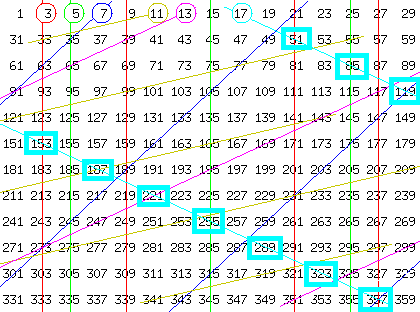
\includegraphics[width=3in]{online-competition-2021-02-18/eratosthenes-with-17.png}}
\[  \begin{array}{rcl}
1/3 & = & \mathtt{0.333333...} = \mathtt{0.(3)},\;\;\text{(periods $T=1$)}\\
1/11 & = & \mathtt{0.090909...} = \mathtt{0.(09)},\;\;\text{(periods $T=2$)}\\
1/37 & = & \mathtt{0.027027...} = \mathtt{0.(027)},\;\;\text{(periods $T=3$)}\\
1/41 & = & \mathtt{0.0243902439...} = \mathtt{0.(02439)},\;\;\text{(periods $T=5$)}\\
1/7 & = & \mathtt{0.142857142857...} = \mathtt{0.(142857)},\;\;\text{(periods $T=6$)}\\
\end{array} \]
\caption{\label{fig:division-samples} Bezgalīgu periodisku decimāldaļu piemēri.}
\end{figure}


\vspace{10pt}
\begin{problem}
Attēlā~\ref{fig:division-samples} redzami vairāku pirmskaitļu apgriezto lielumu $1/p$ decimālpieraksti 
($p = 3,11,37,41,7,\ldots$), kas ir bezgalīgas periodiskas decimāldaļas ar dažādiem 
periodiem. Atrast mazāko pirmskaitli $p$ ar īpašību, ka $1/p$ ir periodiska decimāldaļa
ar periodu $T=4$ (viena un tā pati četru ciparu grupa bezgalīgi atkārtojas).

{\bf Jautājums:} Ierakstīt pirmskaitli $p$ ar minēto īpašību.
\answer{

{\bf Atbilde:} $\mathtt{101}$\\
Dalīšanas rezultāts ir $0.00990099\ldots = 0.(0099)$. 

Ievērosim arī, ka $1/9999 = 0.00010001\ldots = 0.(0001)$. 
Tāpēc $p = 101$ ir vienīgais pirmskaitlis ar šādu periodu, jo 
tam jābūt skaitļa $9999$ dalītājam, lai daļu 
\[ \frac{a}{9999}=\frac{1}{101}. \]
varētu saīsināt vienalga kādam veselam skaitlim $a$. (Šajā gadījumā $a=0099 =99$.)

Bet $9999 = 3^3 \cdot 11 \cdot 101$. Tāpēc vienīgais pirmskaitlis ar šo periodu ir 
$101$, jo skaitļi $1/3$ un $1/11$ dod īsākus periodus. 
}
\end{problem}



\vspace{10pt}
\begin{problem}
Lielākais šobrīd zināmais pirmskaitlis ir $2^{82\,589\,933} - 1$ (pirmskaitļus, kas izsakāmi kā $2^p-1$ 
sauc par Mersena pirmskaitļiem).
Miķelītis uzrakstīja vēl lielāku skaitli $N = 2^{82\,589\,934} - 1$, kuram kāpinātājs 
$82589934$ dalās ar $3$. Miķelītis uzskata, ka uzrakstītais $N$ arī ir pirmskaitlis un pārspēj zināmo pasaules rekordu. 
Pamatojiet, ka Miķelītim nav taisnība.

{\bf Jautājums:} Ierakstīt atbildē mazāko pirmskaitli $p<N$, ar kuru noteikti dalās $N$.
\answer{

{\bf Atbilde.} $\mathtt{3}$ (\textcolor{orange}{1 punkts})\\
{\bf Daļējās atbildes.} Kā ne-mazākais pirmskaitlis der $\mathtt{7}$ vai $\mathtt{2\^{}1966427-1}$ u.c. (\textcolor{orange}{0.5 punkts})\\
Pamatosim, kāpēc tās der.
Tā kā kāpinātājs $82589934$ dalās ar $3$, tad $N = 2^{3k}-1$ var dalīt reizinātājos, izmantojot ģeometriskās progresijas summas formulu. 

Vispārīgā ģeometriskās progresijas summas formula ir šī algebriskā identitāte: 
\[ a^k - b^k = (a-b) \cdot \left( a^{k-1} + a^{k-2}b + \ldots + ab^{k-2} + b^{k-1} \right), \]
kas ir līdzvērtīgi citai izteiksmei:
\[ \left( a^{k-1} + a^{k-2}b + \ldots + ab^{k-2} + b^{k-1} \right) = \frac{a^k - b^k}{a-b}. \]

Mūsu gadījumā $k = 27529978$, $a = 2^3$ un $b = 1$. Tad 
\[ N = 2^{82589934}-1 = \left( 2^3 \right)^{27529978} - 1^{27529978} = \left( 2^3 - 1 \right) \cdot \left( \left( 2^3 \right)^{k-1} + \left( 2^3 \right)^{k-2} + \ldots + 1 \right). \]
Tātad $N$ dalās ar $2^3 - 1 = 7$. 

Bet kāpinātāju $82589934$ var dalīt reizinātājos arī citādi. Tas dalās arī ar $2$. Tādēļ  
\[ N = 2^{2k}-1 = (2^2)^k-1  = (2^2 - 1)((2^2)^{k-1} + \ldots + 1). \] 
No šejienes $N$ dalās ar $2^2 - 1= 3$ (sanāk, ka $p=3$ ir mazākais pirmskaitlis, kas dala $N$).

Var dalīt vēl daudzos citos veidos, teiksim, $N = 2^{42k} - 1$, no kurienes $N$ dalās ar $2^{42} - 1$ utml.
}
\end{problem}





\end{document}



\begin{thebibliography}{1}

\bibitem{Milas2015} Antun Milas. SUNY University of Albany. Abstract Algebra AMAT 327 (2015).
Review Exam, Problem 3. Savākts no \url{https://bit.ly/37fSHN2}.

\bibitem{Raji2020} Wissam Raji. Elementary Number Theory (Ch4.2. The Number-of-Divisors Function). American University of Berut. 2020. 
Savākts no \url{https://bit.ly/2OT820P}. 

\bibitem{Raji2020B} Wissam Raji. Elementary Number Theory (Ch4.2. The The Sum-of-Divisors Function). American University of Berut. 2020. 
Savākts no \url{https://bit.ly/3dS6iiW}.

\bibitem{UTMprimeGaps} Table of Known Maximal Gaps. {\em University Tennessee at Martin}. Savākts no \url{https://bit.ly/3k2Kimo}.

\bibitem{WolframAlpha} WolframAlpha Web service. Sk. \url{https://www.wolframalpha.com/}.
\end{thebibliography}




\end{document}









